\documentclass[tikz, dvipsnames]{standalone}

\usepackage{mathtools}
%\usepackage{amssymb}

\begin{document}
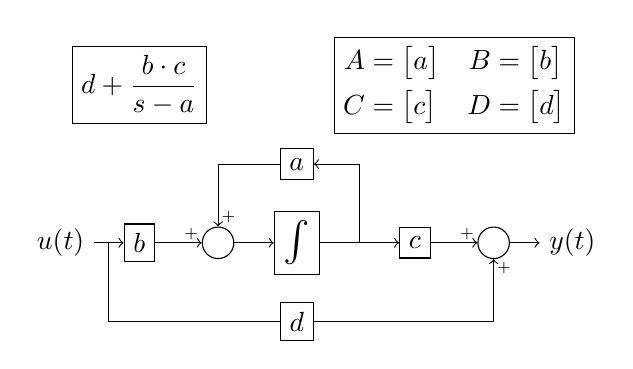
\begin{tikzpicture}
\coordinate (A) at (0,0);
\coordinate (G) at (1,0);
\coordinate (B) at (2,0);
\coordinate (C) at (3,0);
\coordinate (D) at (4,0);
\coordinate (E) at (3,1);
\coordinate (F) at (6.5,0);
\coordinate (H) at (4.5,0);
\coordinate (X) at (5.5,0);
\coordinate (Z) at (1,2);
\coordinate (W) at (5,2);
\coordinate (Y) at (5.5,0);
\coordinate (K) at (3,-1);

\node (Z1) at (Z) {$\boxed{d + \frac{b\cdot c}{s-a}}$};
\node (W1) at (W) {$\boxed{\begin{aligned}A&=\begin{bmatrix}a\end{bmatrix} & B&=\begin{bmatrix}b\end{bmatrix}\\C&=\begin{bmatrix}c\end{bmatrix} & D&=\begin{bmatrix}d\end{bmatrix}\end{aligned}}$};


\node[rectangle,draw] (G1) at (G) {$b$};
\node[rectangle,draw] (H1) at (H) {$c$};
\node[anchor=center] (A1) at (A) {$u(t)$};
\node[circle,draw,inner sep=0pt,minimum size=4mm] (B1) at (B) {};
\node[circle,draw,inner sep=0pt,minimum size=4mm] (X1) at (X) {};
\node[rectangle,draw] (C1) at (C) {\Large $\int$};
\node[rectangle,draw] (E1) at (E) {$a$};
\node (F1) at (F) {$y(t)$};
\node[rectangle,draw] (K1) at (K) {$d$};
\draw[->] (A1) -- (G1) coordinate[midway] (I);
\draw[->] (I) --++(0,-1) --(K1) -| (X1) node[pos=1,anchor=north west, inner sep=1pt] {\tiny $+$};;
\draw[->] (G1) -- (B1) node[pos=1,anchor=south east, inner sep=1pt] {\tiny $+$};
\draw[->] (B1) -- (C1);
\draw[->] (E1) -| (B1) node[pos=1,anchor=south west, inner sep=1pt] {\tiny $+$};
\draw[->] (C1) -- (H1) coordinate[midway] (J);
\draw[->] (J) |- (E1);
\draw[->] (H1) -- (X1) node[pos=1,anchor=south east, inner sep=1pt] {\tiny $+$};
\draw[->] (X1) -- (F1);

\end{tikzpicture}
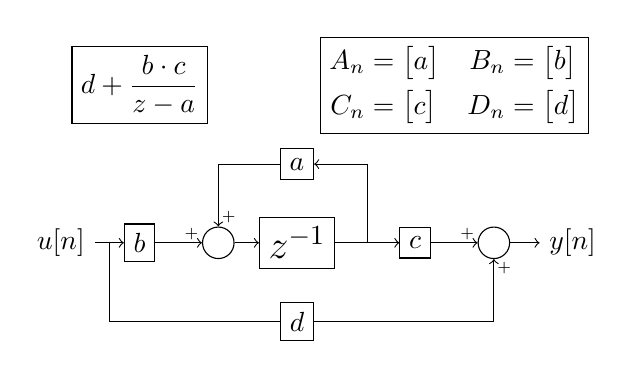
\begin{tikzpicture}
\coordinate (A) at (0,0);
\coordinate (G) at (1,0);
\coordinate (B) at (2,0);
\coordinate (C) at (3,0);
\coordinate (D) at (4,0);
\coordinate (E) at (3,1);
\coordinate (F) at (6.5,0);
\coordinate (H) at (4.5,0);
\coordinate (X) at (5.5,0);
\coordinate (Z) at (1,2);
\coordinate (W) at (5,2);
\coordinate (Y) at (5.5,0);
\coordinate (K) at (3,-1);

\node (Z1) at (Z) {$\boxed{d + \frac{b\cdot c}{z-a}}$};
\node (W1) at (W) {$\boxed{\begin{aligned}A_n&=\begin{bmatrix}a\end{bmatrix} & B_n&=\begin{bmatrix}b\end{bmatrix}\\C_n&=\begin{bmatrix}c\end{bmatrix} & D_n&=\begin{bmatrix}d\end{bmatrix}\end{aligned}}$};

\node[rectangle,draw] (G1) at (G) {$b$};
\node[rectangle,draw] (H1) at (H) {$c$};
\node[anchor=center] (A1) at (A) {$u[n]$};
\node[circle,draw,inner sep=0pt,minimum size=4mm] (B1) at (B) {};
\node[circle,draw,inner sep=0pt,minimum size=4mm] (X1) at (X) {};
\node[rectangle,draw] (C1) at (C) {\Large $z^{-1}$};
\node[rectangle,draw] (E1) at (E) {$a$};
\node (F1) at (F) {$y[n]$};
\node[rectangle,draw] (K1) at (K) {$d$};


\draw[->] (A1) -- (G1) coordinate[midway] (I);
\draw[->] (I) --++(0,-1) --(K1)  -| (X1) node[pos=1,anchor=north west, inner sep=1pt] {\tiny $+$};;
\draw[->] (G1) -- (B1) node[pos=1,anchor=south east, inner sep=1pt] {\tiny $+$};
\draw[->] (B1) -- (C1);
\draw[->] (E1) -| (B1) node[pos=1,anchor=south west, inner sep=1pt] {\tiny $+$};
\draw[->] (C1) -- (H1) coordinate[midway] (J);
\draw[->] (J) |- (E1);
\draw[->] (H1) -- (X1) node[pos=1,anchor=south east, inner sep=1pt] {\tiny $+$};
\draw[->] (X1) -- (F1);

\end{tikzpicture}
\end{document}